% !TeX spellcheck = en_GB

\subsection*{Search Terms TOTAL PAGES 5/69}
portal
3D lense
magic lense
Seams

dual depth buffer
Walkthrough applications
Transformative Portal
\section{Introduction 0/1}

\subsection{Disambiguation}
portal in a game
vs
portal as occlusion culling

\section{Literatur 0/15}

\subsection{Portals as Occlusion Culling}
potentially visible set
\cite{luebke:1995:portals}
\cite{yang:2014:walkthrough}

\subsection{Portals Algorithms History}


Portal Rendering in SEAMS (\cite{schmalstieg:1999:sewing})

Complex Portal rendering. (I use the same near Buffer technique) \cite{ lowe:2005:technique}


\url{https://th0mas.nl/2013/05/19/rendering-recursive-portals-with-opengl/}
\subsection{Portal Applications}

\subsubsection{Magic Lense}
\cite{viega:1996:3d}


\subsubsection{VR Interaction 3D Lenses}
\cite{borst:2009:real}
3D lenses which change, the properties. E.g. other rendered objects (x ray lense), inverted colors, fish eye effect.

\subsubsection{Navigation}
Portal Rendering in SEAMS (\cite{schmalstieg:1999:sewing})
\cite{pausch:1995:navigation} navigation with hand held minatures


\subsubsection{Game Mechanik}
Portal, Antichamber, Splitgate Warfare Arena

\subsubsection{VR Movement}

Portal Locomotion in Budget Cuts\url{https://www.youtube.com/watch?v=f786ak3GKQo}

\subsubsection{Fit More Space in Less Space}

\subsubsection{Space Division}
Rooms are split by portals. For each portal only the objects in its room need to be drawn.
\cite{ lowe:2005:technique}

\subsection{Graphics Programming 0/9}


\subsubsection{Raytracing}
software,
gpu,
NVIDIA RTX cards, Ray shaders?

\subsubsection{Rasterization}

\subsubsection{GPU Synchronisation}

\subsubsection{Uniforms / Storage Buffer Objects}

\subsubsection{Shaders / (Vulkan-) GLSL / SPIR-V}
branching, fragment discard, early stencil / depth, force early test, Stencil Export

\subsubsection{Occlusion Queries}

\subsubsection{OpenGL}
History


\subsubsection{Vulkan Overview}
input attachments, tile renderers,

(Sub-)Renderpass, Push Constants, Validation Layers, Pipelines, Dynamic state,

Molten VK-Framwork

\subsubsection{Depth / Stencil Test}
Limitations, common uses
Early Z! Fragment discard
Z Fighting,
Depth Formtas
inverse depth buffer with floating point is magic!

combined depth / stencil
\url{https://developer.nvidia.com/content/depth-precision-visualized}

\subsubsection{Push Constant}

\subsubsection{Instanced Drawing}

\section{Implementation 5/30}

\subsection{Technologies / Libraries}
SDL, glm, vulkan, rapid xml, c++, vulkan memory allocator

\subsection{Software Raytracing 0.5}
The first implementation was based on software raytracing. Compared to rasterization based methods, raytracing allows for more complex operations on individual rays. A response to an instersection can spawn a new ray, which replaces the old ray. The new ray can have many different properties. The new ray can have an completely different origin and direction, which would simulate a portal. Additionally a non conventional ray definition could be used, allowing for bent rays. Rays could travel slower, resulting in scaled space.

The prototype was implemented in C++ using SDL \cite{SDL} and GLM \cite{GLM} as libraries. It performs an intersection test against sphere. The ray line intersection query uses the algorithm described by \textcite{eberly:2006:3d}. Additionally, the pixels of the SDL Surface were manipulated directly instead of using an SDL Renderer to improve performance.

Even with this simple test, the prototype performed poorly. A scene with only one sphere took more than 40 milliseconds to render on a 1920x1080 resolution. When subtracting the time needed to render an empty scene, it still takes over 20 milliseconds. For realtime applications it is completely unviable.

There are still some improvement opportunities with multithreading, rendering to smaller resolutions, and using simpler tests. However, with an high render time already this high, continuing seemed to risky and this approach was abandoned.

%TODO Include Measurements and PC Stats?

\subsection{Why Vulkan 0.5}
One important aspect of the prototpye was that it can run on as many plattforms as possible. %TODO: Should / Where Should it state the reason for supporting more plattforms
For graphic \glspl{api} this restricts the set of options to OpenGL and Vulkan. Apple recently announced the end of its OpenGL support \cite{arstechnica:openGL}. Vulkan is not directly supported by Apple. However, it is possible to use still OpenGL and Vulkan on Apple products, using MoltenGL \cite{moltenGL} and MoltenVK \cite{moltenVK} respectively. Both \glspl{api} are safe to use for a foreseeable time.

Vulkan is much more explicit and low level compared to OpenGL. This allows for more room to optimize. However, this also means that Vulkan is also more verbose and it takes longer to get started.

OpenGL is a stateful \gls{api}. It has a global state which can be manipulated with function calls. Vulkan is stateless, all functions manipulate a given object. While it easier to get started with global state, it is more difficult to maintain the bigger the project gets.

As the implementation of the prototype is expected to take quite a while, and might be further worked on after this thesis. With maintainability and optimization possibilities as important concern, Vulkan is more suitable for the project. 
%TODO: subjective why vulkan
(Subjective Reason: Want to learn vulkan?) 

\subsection{Terminology}

\subsubsection{Portal}
Portals are defined as 2 Objects/Endpoints which share a mesh. The both endpoint may have any transformation. From those two endpoints, two teleportation matrices are generated, which when applyied move an object from one end point to the other.

Instead of an mesh representation, other representations, could have been used. E.g. A spehre which is defined by a mathematical equation.

\subsubsection{Portal Pairs and endpoints}
A Portal pair are two portals, which are connected with each other. The induvidual portals of a pair are called endpoints. If an object moves through one endpoint, it is teleported to the other. The connection is two way, allowing back and forth movement teleportation. 



\subsubsection{Camera Matrix}
The camera is defined by a camera matrix. It is similar to a modelmatrix. The inverse of the camera matrix is the view matrix which is used to render the scene.
%%\subsubsection{Transform}
%%A transform defines an objects attributes such as translation, rotation or scale. A transform can be applied to a point, as well as other transforms. 


\subsection{Textures vs Stencil Buffer 0.5}
\label{section:textursVsStencil}
Two different approaches were considered to render the contents of a portal. The first approach is to render the scene from the portal's viewpoint to a texture in the first renderpass. In the next renderpass this texture is applied to the portal and the scene is then rendered as usual \cite{lecture:portalProblems}.  %TODO: find source

The other approach utilises the stencil test. The stencil test is initially set to always pass. First the scene is drawn without portals.
The the portals are draw. For this renderpass, the stencil operation must be set in a way to mark the visible portal pixels. Now at least the depth values for visible portal pixels must be cleared. It is also possible to clear the whole buffer. Next step is to move the camera to the portal's viewpoint. Finally the scene is drawn again, but pixels that are not marked are discarded \cites{schmalstieg:1999:sewing, lowe:2005:technique, lecture:portalProblems}.

For both approaches care must be taken to discard fragments that are between the portal's viewpoint and the portal exit. With multiple visible portals, the steps which use the portals viewpoint, must be executed at least per visible portal. Additionally it must be ensured, that each portal has the correct contents.

This implementation uses the latter approach, as it does not need extra textures. Especially considering recursions, the first approach might need many textures and do not need the stencil buffer for anything else.

\subsection{Generating Camera Matrices 1.6}
As describe in section \ref{section:textursVsStencil} the camera needs to be move to the portals view point. However, this is no fixed location and depends on the current camera position.

\begin{figure}[h]
	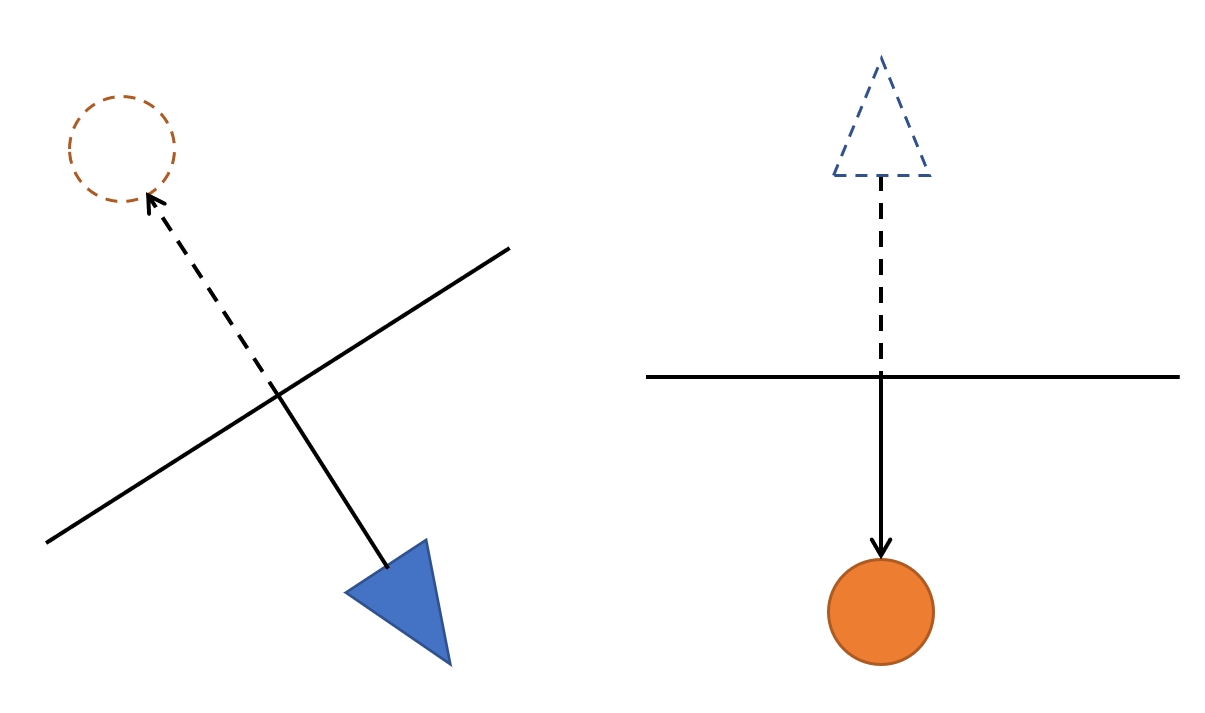
\includegraphics[width=\linewidth]{images/camera_matrices.png}
	\caption{Portal Camera}
	\label{fig:cameramatrices}
\end{figure}

Figure \ref{fig:cameramatrices} shows two portal endpoints. The blue triangle represents the camera and the orange circle represents an objects. The dotted blue triangle represents the portal view camera.
When looking through the portal, it must look as if the camera looks directly a the object. After a camera matrix is calculated, the view matrix can be obtained by inverting it.

\subsubsection{Initial Approach 0.2}
The initial approach first calculates the vector from the visible Portal Endpoint location to the camera. Then rotates that vector by the rotation difference of the two endpoints. Finally that vector gets added to the other Endpoint location. This is new camera origin.
To calculate the portal view camera rotation, the original camera's rotation is multiplied by the rotation difference between the two endpoints.
The initial approach did only consider rotations and translations.

\subsubsection{Current Approach - Teleportation Matrix 0.3}
The current approach uses coordinate transforms to calculate the portal view camera. By applying the inverse modelmatrix of endpoint A to the camera matrix, we bring the camera in a coordinate system, where endpoint A is at the origin. The camera matrix is now expressed relative to endpoint A. Finally we can apply Endpoint B's which moves exactly at the right position relative to endpoint B.
For example if the current camera's location where exactly at endpoint A, applying the inverse modelmatrix of endpoint A would move it to the origin.
The Application of the two matrices can be combined into one. The implementation this is called the teleportation matrix. It is also used to move objects from one end point to the other.  

%TODO other analogy? Relative attachments in scenegraphs? 

\subsubsection{Recursive Portal Matrices 0.75}
The previous sections explained how to calculate the camera matrices for each portal. However, for recursion we need to calculate the camera transforms for any combination of portals. This can be achieved by using the same approach multiple times, applying it on the result of the previous iteration. This is needed for each combination of portals. For each iteration we need an addition M matrices, where M equals the number of portals to the power of the current iteration. If there are 4 portals, the initial scene rendering would need 1 matrix, the camera matrix. Iteration 1 would need 4 additional, one for each portal. Iteration 2 would need 16 portals, 1 for each possible portal pair. With two iterations a total of 21 matrices are needed.

The view matrices are stored in one continuous array, but has a tree-like inner structure. The root is the current view matrix. Each child contains to the corresponding portal's view matrix, relative to its parent matrix. The indices can be found the following way:

\begin{itemize}
	\item $ nth child = current index * portalcount + 1 + n$
	\item $ parent = \lfloor(current index-1)/portal count\rfloor $
\end{itemize}

%%$c_n .. nth child index$
%%$p .. parent index$
%%$i ... curent index$
%%$t ... portal count$




\begin{figure}[h]
	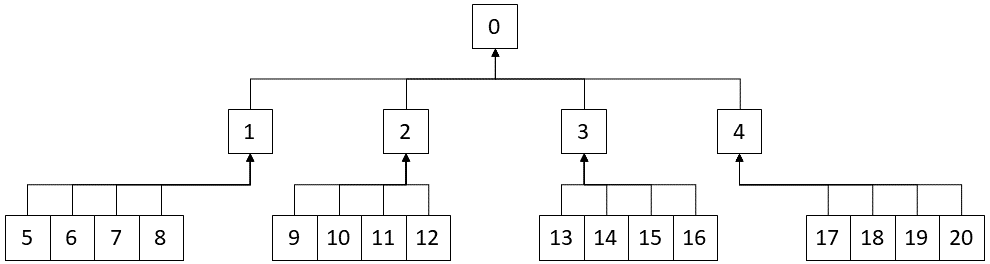
\includegraphics[width=\linewidth]{images/cameraindices.png}
	\caption{Camera Indices}
	\label{fig:cameraindices}
\end{figure}

Figure \ref{fig:cameraindices} shows the indices for 4 portals, with 2 iterations. For example to find the view matrix of Portal 0, seen through Portal 1, we would access the array at index 9.


\subsection{Portal drawing orderer Depth first vs breadth first 1.25}

\begin{figure}[h]
	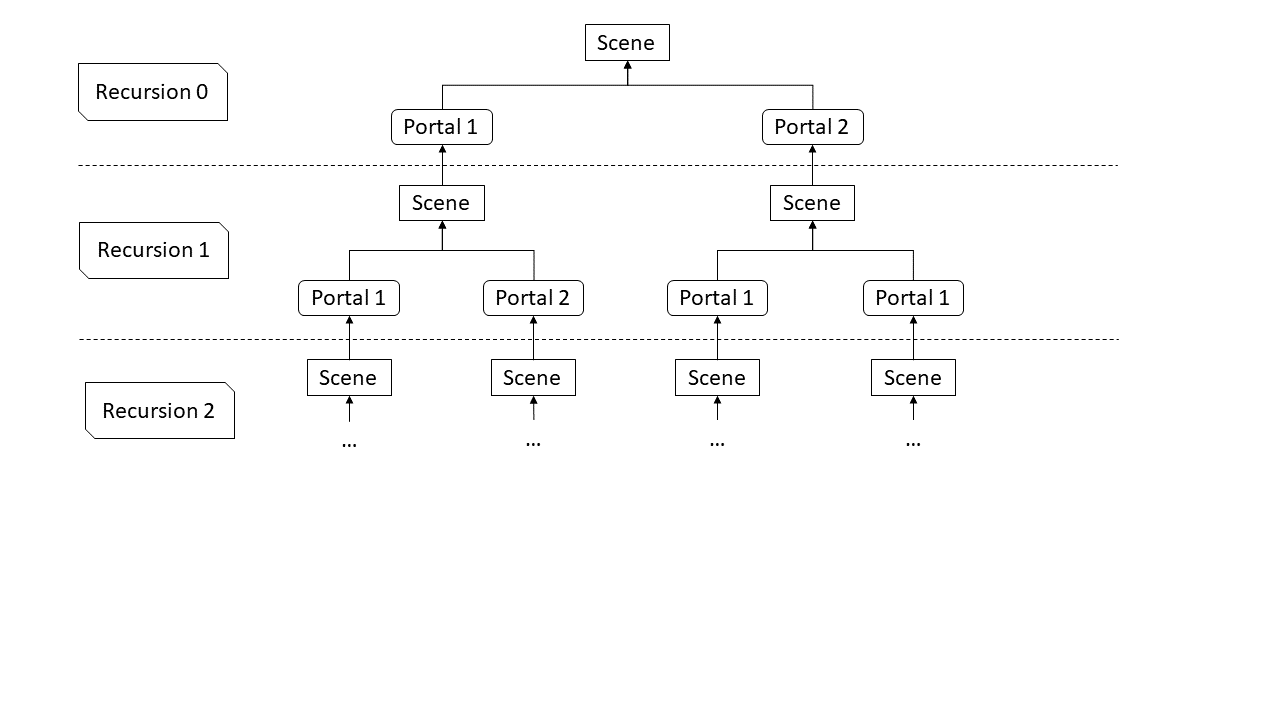
\includegraphics[width=\linewidth]{images/rendertree.png}
	\caption{Render Dependencies}
	\label{fig:rendertree}
\end{figure}

When drawing multiple portals recursively the draw dependencies can be imagined as a tree. Figure \ref{fig:rendertree} shows the dependencies for two portals. In recursion 0 the two portals can only be drawn after the scene was drawn. Otherwise portals that are occluded by a scene object might wrongly mark the pixel in the stencil buffer. The two scenes in recusion 1 can only be drawn when their respective portal was already drawn. However, it is not necessary that all portals from recursion 0 were drawn, before a scene from recursion 1 is drawn.

There are two approaches on the drawing order: depth first or breadth first. In depth first the contents of Portal 1 in recursion 0 would be fully complete, before it begins drawing the contents of Portal 2 in recursion 0. This has the advantage of needing just a small amount of different values to mark a pixel. Going down the tree a different value can be used for each recursion. When going up that value is not needed anymore and can be recyled. However, the implementation must make sure that no unneeded value remains in the stencil buffer. A downside is, that the draws are is fully dependent on each other.

Breath first draws a recursion completely before drawing the next recursion. The amount of different values needed to mark a pixel, scales exponentially. It needs one value of each portal in a recursion. For a scene with two portals, to mark all portals from recusion 1 it at least needs 4 different values, excluding 0. For recursion 2 it needs 8 values. With the stencil buffer usually being limited to 8 bits this can be quickly be a hard limit. However, the advantage is that the depth buffer needs to be cleared less often, only when transitioning between recursions. Additionally, within a recursion there are not dependencies between the multiple scene draws, as well as the portal draws.

Previous transformative portal implementations used depth first \cite{lowe:2005:technique,lecture:portalProblems}. The implementation presented in this thesis uses breadth first. Fewer dependencies between the draws could be exploited. Additionally similar draws can be grouped, which reduces the amount of renderpasses. While the amount of stencil values needed scales exponentially, the amount of draws scaled exponentially too. The author believes it is more likely that amount of draws will be the limiting factor than running out of values in the stencil buffer.

\subsection{Dual Depth Buffer 1}

When drawing the scene from the portals view, care must be taken to not draw objects, that are between the camera and other endpoint.
\begin{figure}[h]
	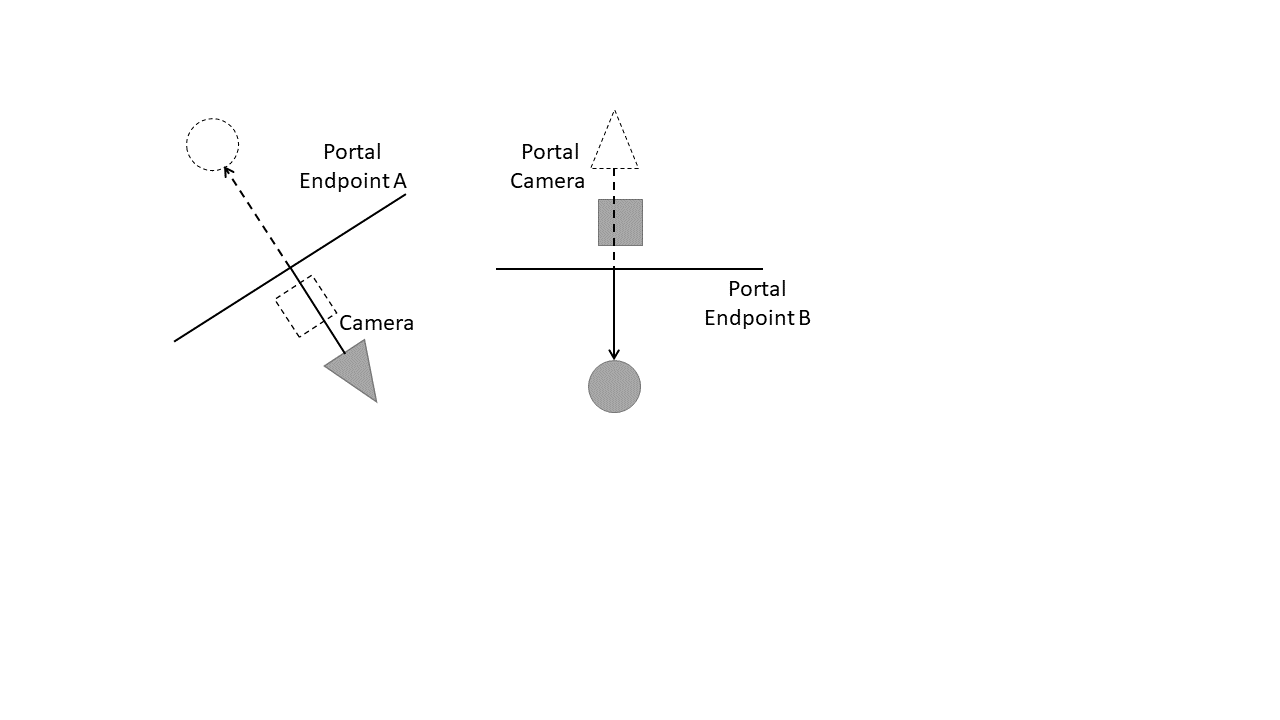
\includegraphics[width=\linewidth]{images/bananajuce.png}
	\caption{Object between portal camera and portal endpoint}
	\label{fig:bananajuce}
\end{figure}

Figure \ref{fig:bananajuce} shows such an example. Without additional techniques the square would be drawn. To avoid this, the implementation uses two depth buffers or dual depth buffer: a near depth buffer and a far depth buffer. The far depth buffer is used to discards fragments with a greater depth value. It is just a regular depth buffer, which is used in almost any rendering system. The near depth buffer discards fragments with a lesser depth value. When rendering the portal we render its depth also to the near buffer. The box's depth values from figure \ref{fig:bananajuce} would be greater than the near buffer and its fragments are discarded \cite{lowe:2005:technique}.

In this implementation the hardware supported depth buffer is used as the far buffer. For the near buffer dual buffering with two color texture are used, a read near buffer and a write near buffer. In the fragment shader, the fragments depth value is compared to the read near buffer. If it is lesser it is manually discarded, with a discard statement in the shader. Whenever the portals are drawn, they not only write the far depth buffer, but also the write near depth buffer. When the implementation transitions to the next recursion, the write near buffer and read near buffers are swapped.

Dual buffering the near buffer avoids problems with edge case where one portal occludes another and the portal behind is drawn first. With only one near buffer, the portal behind would set the near buffer to its value. The fragments of the portal in front would be discarded, instead of occluding the portal behind.

The read near buffer is a input attachment and the write near buffer is a color attachment. In recursion 0, no read near buffer test is used.

\subsection{Portal near Z fighting 0.33}
When rendering the contents of one endpoint of a portal pair, the other endpoint would be rendered directly at the same location. Due to precision errors in floating point calculations, the other endpoint would sometimes be discard by the near buffer and sometimes not. This leads to a special case of Z fighting. To avoid this we store the winding order of a fragment in the near buffer. When the fragments depth value and the near buffer value are nearly equal and winding order is the same, we have exactly the previously mentioned case and need to discard the fragment. This is done by increasing the comparison value by some small amount or percentage for same winding orders.

As the implementation has a depth range of 0 to 1, the value will always be positive. This allows the implementation to store the winding order is store as the sign of the near buffer. Positive values indicating front facing and negative values indicating back facing. Near Depth comparison is done with the absolute value of the buffer.

\subsection{Stencil Values and compare masks 0.66}
\label{section:stencilcomparemasks}

As the implementation uses the breadth first approach, it can not use the stencil increment and decrement technique described by other implementors \cite{schmalstieg:1999:sewing, lowe:2003:fragment, lecture:portalProblems}. Different values need to be stored and compared against. Directly setting the stencil value can be achieve, by setting a reference value and use the replace stencil operation. However, the stencil reference is also used for the comparison. This means that the implementation must be use the same value for comparison as well as writing. This can be achieved by the use of stencil compare mask and generating stencil values with postfixing.

\begin{figure}[h]
	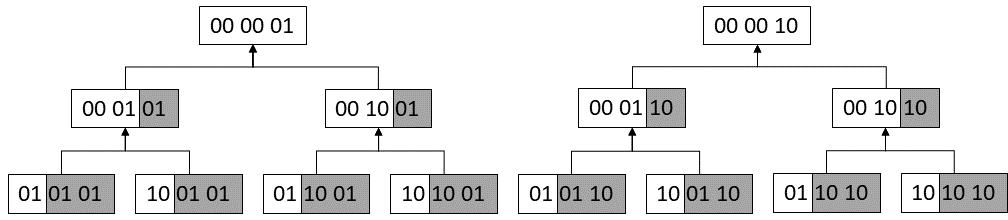
\includegraphics[width=\linewidth]{images/stencilvalues2.png}
	\caption{Compare Mask and Stencil Values}
	\label{fig:stencilvalues}
\end{figure}

Figure \ref{fig:stencilvalues} shows is process with two portals and 6 bits. The grey part is used for comparisions, while the whole value is used to write. The comparision mask of Recusion 0 mask out all bits, so the test will always succeed. For two portals recursion 1 mask out all but the last two bits. Notice that the last two bits of  recursion 1's stencil values are the same as their respective parent values. It is important that stencil values start with 1 and not with 0, otherwise they are not distinguishable from their parent values.

This also means that the range of values is one less than representable by the number of bits. This is very significant, as the portals come in pairs. The number of bits needed for two and four portals is one more than normally needed. As the stencil buffer usually only has eight bits, this limits the amount of recursions considerably.

\subsection{Storing Mesh Data for Rendering}

\subsection{Initial Portal Rendering}

The implementation uses just one renderpass, with multiple subpasses. This allows for the use of input attachments and potentially enables the \gls{gpu} driver to optimize. For example many textured are only needed within the renderpass and do not need to be transferred anywhere else.

\begin{figure}[h]
	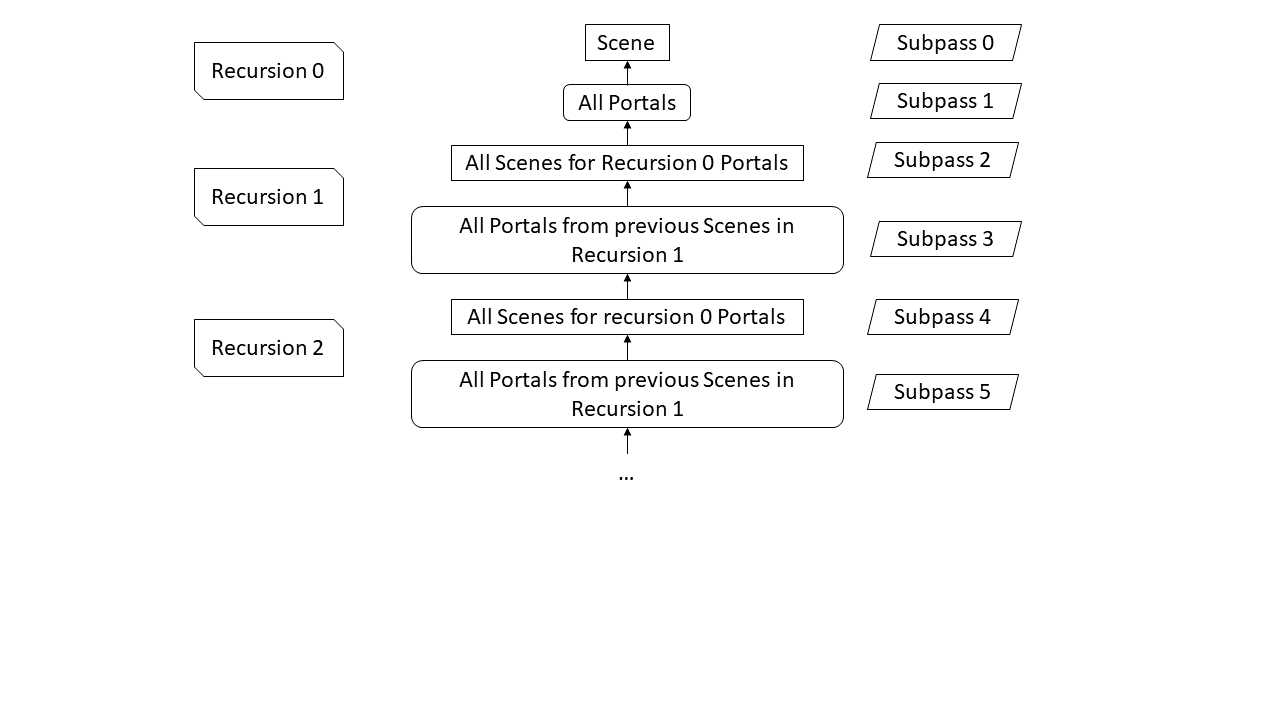
\includegraphics[width=\linewidth]{images/renderpasses.png}
	\caption{Subpasses and work done}
	\label{fig:renderpasses}
\end{figure}

\subsubsection{Renderpass Setup}

Figure \ref{fig:renderpasses} shows the subpasses, which recursion they belong to and what work is done. Notice that compared to figure \ref{fig:rendertree} scene and portal draws are each batched together. Every even subpass is responsible for drawing a scene, while in every odd subpass the portals are drawn. The subpass index divided by two equals the recursion index. 

\begin{figure}[h]
	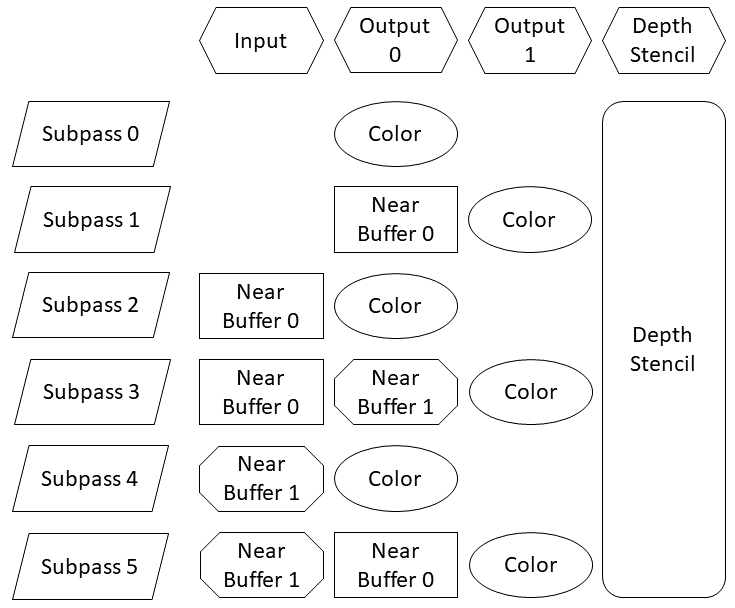
\includegraphics[width=\linewidth]{images/attachmentsetup.png}
	\caption{Attachment Setup}
	\label{fig:attachments}
\end{figure}

Figure \ref{fig:attachments} illustrates the attachments of the individual subpasses for two recursion. Odd subpasses write into the near buffer, which is used as input for the following two subpasses. For a real application portals do not need to write color so output 1 is not really needed. However, for this implementation it is kept for debugging purposes.
The last subpass does not need to write to the near buffer, as there are not later subpasses which could use it. It is kept for debugging purposes too. The depth stencil attachment is never changed. The color and depthstencil attachment are cleared at the beginning of the renderpass with VK\_ATTACHMENT\_LOAD\_OP\_CLEAR. Both near buffers use VK\_ATTACHMENT\_LOAD\_OP\_DONT\_CARE. The stencil test ensures that they are only accessed at locations where portals have previously written a value. Each subpass has set a dependency in the fragment shader on the previous subpass' output.


\subsubsection{Graphic Pipelines}
When rendering the multiple scene one after each other, as well as when rendering the portals, the stencil reference needs to be changed. There are two options how to resolve this problem: either using multiple pipelines or using dynamic pipeline state. For the implementation dynamic pipeline state was used, as the number of graphic pipelines needed would scale exponentially with the amount of portals and recursions. Dynamic state seemed much easier to manage in comparison.

However, the subpass index cannot be dynamic state. Thus even with dynamic stencil references, there must be at least the same amount of graphic pipelines as there are subpasses. If more than one shader is used for rendering scene objects or portals, the amount of graphic pipelines is increased. Each additional shader increase the amount by half of the subpass amount, as it is either only used for portal rendering or only for scene rendering. As there already are different pipelines for the subpasses, each of them can have a different stencil compare mask (see section \ref{section:stencilcomparemasks}). There is no need for dynamic stencil compare masks.

One important aspect is that pipelines for both scene and portal drawing, have face culling disabled. Portals do not have to be watertight and scene object might be transformed in a way that changes winding order. If it can be ensured that there are no teleportation matrices that change winding order, then face culling could be enabled for scene objects. For this implementation it was chosen to support such teleportation matrices.

The individual  graphic pipelines for drawing the scene differ only by subpass index and stencil compare mask. Otherwise they are the same. This is also true for the graphic pipelines for portal drawing.

\subsubsection{Shaders}

\subsubsection{Draw Order}

In subsequent draws, perform stencil test as well as test against "rendered depth" (similar to clip plane used in Portal 2).
We can force early depth/stencil as we never draw a pixels if it failes the test. We only maybe discard it if the test succeds.

Use pushconstant to decide camera index
clear depth between iterations
use dynamic stencil ref and stencil compare mask, to cut down number of pipelines drastically. Might not be optimal?


\subsubsection{Properties}
fixed number of portals, scales poorly
stencil values known at compile time
Not flexible
Very limited amout of portals an recursions

\subsection{Dynamic Portal Rendering}
Camera matrices are not accessed directly. Instead an an array is accessed which stores the id. Allows to dynamically change camera matrices
Invalid ids means we can skipp that draw -> Set all values in vertex shader to same value to create a degenerate triangle, to improve performance.
Calculate portal Id, dicard if portal id is greater than visible portals
Use portal Id to generate stencil value and the camera id.


\subsubsection{Visible Portal Number algorithm}
in fragmentshader: counter, traverse array, increase for non zeros, ignore at index corresponding to the current portal
write own number or 1 at the ignored location -> Multiple writes of same value should be save, accross "threads", when counting this is skipped so we have no reader at the moment
Needs synchornisation so that value is visible for the next portal!
-> Pseudo occlusion query with immediate result.
-> very conservatic. Portals totaly occluded by later portals or discarded by stencil test still counts as "visible". We can't check for stencil failure, as we can't access the stencil buffer.
-> depth prepass could mitigate this

\subsubsection{Occlusion query alternative}
probably slow
needs to process portals and then again with the result
probably needs some extra throwaway texture

\subsubsection{Properties}
fixed number of visible portals in each portal, which can be dynamic for recursion. E.G inital 4 visible portals, but in each of those only 2 visible portals
Number can be changed at runtime.
Even if visible portal count is too high, we can at least only produce degenerate triangles to save performance.

Requires stencil export (!). Not supported on nvidia cards (source: \url{https://vulkan.gpuinfo.org/listdevices.php?platform=windows&extension=VK_EXT_shader_stencil_export})
No early test for Portal rendering, as we are using stencil export.



\subsection{Dynamic Portal instance rendering}
We render objects for each rendered portal of previous pass. Only difference is stencil value and camera index.
Camera Index can be calculated with InstanceIndex
Can't change stencil during instance drawing -> Drop Stencil Test. Use extra texture an perform it manually in shader, similar to rendered depth test. 

\subsubsection{Properties}
No early test for Scene.
Recursion and Portal count is only limited by performance, as we can use any number of bits for our test.
Number of draw calls now scales linearly with recursion count (although actuall draw count remains the same).
No Need for Stencil prefixes -> simplifies code, saves bits

Huge Performance Improvement!!! Was 6 times fast in my case. 
(should I measure this and create diagram?)




\subsection{Portal Collision}
On portal collision we apply the same operation on the camera, that would be applied to an object rendered through that portal.
It is implemented by storing a matrix of cumulative portal teleport matrices.
However, it is also possible to apply only a part of it for some interesting effects, but it will result in non seamless translation.

\subsection{Collision Detection (??)}
Raytrace with triangles (could be improved)
KD trees
Surface area heuristic

\subsection{Player Rendering}
When looking through a portal, players might see themselves. Care must be taken when rendering. Standing directly in fron of the portal and touching it slightly could make the player see their only model at their own location. (see valve talk \url{https://www.youtube.com/watch?v=riijspB9DIQ})



\subsection{Face Culling}
Appying face culling only works if no portal changes the scale of an object. Otherwise the triangle order gets changed too and wrong side will be rendered.

\subsection{Level Editor}
Ideally a custom level editor should be built, so the effect of the portals can be seen immediately. However, there was not enough time. After looking for various solution, using the unreal engine seemed best, as the author has some experience with it.

The UE4 Level editor is very convenient and can be customized. The level is exported with a Editor Script. However, some care must be taken as UE4 has a different coordinate system. For Vectors Y and Z must be swapped. For Quaternions, y and z must be swapped and the imaginary part inverted, as we are changing handedness.


\section{Analysis And Improvements 0/15}

\subsection{GPU Raytracing}

\subsection{Camera Matrix Improvement opportunities}
Could be improved. The work to calculate the matrices scales super linear. $X^{N}$, where X is the portal count and N is the number of iterations.
Instead of precomputing all combinations, it is probably better to calculate the matrices on demand in the fragment shader, as we have much more information there. This saves unnessary computes, removes an indirection and puts the work on the gput. Only downside is that the computation is executed multiple, once per shader fragment. Finally save on bandwith, as they don't need to be transfered!

\subsection{Scaling measurement}

\subsection{Watertight Portals}
Objects behind watertight portals, will look as though that portal did not exist. Portals inside on endpoint of an watertight portals, will be visible when looking at the other endpoint, with the teleportation matrix applied. If watertight portals are static, they are essentially useless. The same scene could have been created without them.
However if they change or are created during runtime they can have interesting effects. Such as Scaling objects, or swapping two areas.

\subsection{Dynamic Portals Instance Rendering}

\subsubsection{Opportunity: Dynamic Visible Portals count}
If we can detect the initial pass only has few visible portals (e.g. via frustrum culling like techniques), we lower the amount for the initial rendering, and increase it for
the subsequent pass.

Handles case of directly standing in front of a portal!
Have not implemented this

\subsubsection{Opportunity: Draw Indirect}
Using draw Indirect allows us to only use one draw call per pass, instead of one per object!
Additionally we can manipulate the draw indirect buffer, while calculating the portal id, so that the instance count matches the amount of actually drawn portals.
This way instead of producing degenerate triangles, we don't even draw meshes.
However, could be problematic as we would need to set each value in the shader, having a loop for each scene element, and many writes.

The conditional execution extension could be used (VK\_EXT\_conditional\_rendering) but only to disable drawing entirely, if no portal is rended -> probably not useful.

\subsubsection{Skip instances}
One downside is, that draw instanced draws the object for each portal. However sometimes would could know, that the object is not visible from a specific Portal, e.g. via Potentially visible set tests, or knowing by other means that the portal will never draw that object (e.g. diffrent world layers).
To combat this problem, we could decrease the draw instances count and provide iformation which portals should be skipped.

Instead of using instanceId directly, this skip information will be used to calculate the real id. The rest would behave the same, just using this genreated id instead of instanceId directly.



\subsection{Non-Translating Portals}
The implemented portals have two endpoints. Objects Touch on endpoint, get move to the other. However, it is also possible that the portals don't move the object. In this case there are no two end points. It is just one portal.

Entering the portal would apply one operation (e.g. multiplying by matrix), leaving it applies the inverse operation. Back and Frontface detection needs to be used to decide which operation to apply.


This only works for operations which don't move the possition of an object, unless it is just an rotation and the portal shape looks the same after applying the rotation to it. E.g. a sphere could allow for any rotation. A cube only for rotation in intervals of 90 degrees.
Changing the scale of an objects would also work, but it is important, the the origin remains a the same position. However, this would result in non seamless portal transitions.

Furthermore, more than just transform can be applied. Operations described in the section \ref{more than transforms} would also work.



\section{Further Work 0/5}
\subsection{Transparent Objects}
\subsection{Shadows}
Without currect handling, we can see portal locations, as shadows would be cut of.
\subsection{lighting}
Without correct lighting seams would be visible. Proabably very difficult for spot/pointlights. Directional light already works.
\subsection{Collision Detection}

\subsection{More than just transforms}
\label{more than transforms}
The current approach uses camera indices, to decide which camera matrix gets applied. However, this approach is not limited to only changing matrices. Inspired by \cite{borst:2009:real} indices could be used to change other paramteres. We could add objects that only render if specific parameters are set, mark pixels for a later post process. Or take as specific branch in any shader.


\subsection{Use the Instant Occlusion query in occlusion culling}
we can set conditional rendering paramters during this occlusion culling.
Needs some  recursive portal passes and then one big scene pass, which makes use of conditional rendering, eitehr with the extension or draw indirect and instance counts. Inspired by \cite{yang:2014:walkthrough}

\section{Conclusion 0/3}

summary
instant pseudo query and other important topics
economic effekt

\section*{stuff}
For debugging OpenGL offers debug output to obtain details about errors, performance warnings and other useful information. They can be obtained via a debug message callback or by querying them from a message log \cite{khronos:openGL:spec4.6}. In Vulkan validations layers are used for finding errors. In Vulkan \gls{api} calls can be intercepted by layers. They perform whatever operation defined by their implementation before maybe passing them to the actual function. Validation layers are layers w

They validate the parameters, before passing them to the actual function. How errors are reported depends on the implementation of the layer.. Multiple layers can be active and are called each one sequentially before calling the actual function. \cite{khronos:vulkan:spec1.1}












